% Options for packages loaded elsewhere
% Options for packages loaded elsewhere
\PassOptionsToPackage{unicode}{hyperref}
\PassOptionsToPackage{hyphens}{url}
\PassOptionsToPackage{dvipsnames,svgnames,x11names}{xcolor}
%
\documentclass[
  12pt,
  a4-paperpaper,
  DIV=11,
  numbers=noendperiod]{scrartcl}
\usepackage{xcolor}
\usepackage{amsmath,amssymb}
\setcounter{secnumdepth}{-\maxdimen} % remove section numbering
\usepackage{iftex}
\ifPDFTeX
  \usepackage[T1]{fontenc}
  \usepackage[utf8]{inputenc}
  \usepackage{textcomp} % provide euro and other symbols
\else % if luatex or xetex
  \usepackage{unicode-math} % this also loads fontspec
  \defaultfontfeatures{Scale=MatchLowercase}
  \defaultfontfeatures[\rmfamily]{Ligatures=TeX,Scale=1}
\fi
\usepackage{lmodern}
\ifPDFTeX\else
  % xetex/luatex font selection
  \setmainfont[]{Open sans}
  \setsansfont[]{Open sans}
\fi
% Use upquote if available, for straight quotes in verbatim environments
\IfFileExists{upquote.sty}{\usepackage{upquote}}{}
\IfFileExists{microtype.sty}{% use microtype if available
  \usepackage[]{microtype}
  \UseMicrotypeSet[protrusion]{basicmath} % disable protrusion for tt fonts
}{}
\usepackage{setspace}
\makeatletter
\@ifundefined{KOMAClassName}{% if non-KOMA class
  \IfFileExists{parskip.sty}{%
    \usepackage{parskip}
  }{% else
    \setlength{\parindent}{0pt}
    \setlength{\parskip}{6pt plus 2pt minus 1pt}}
}{% if KOMA class
  \KOMAoptions{parskip=half}}
\makeatother
% Make \paragraph and \subparagraph free-standing
\makeatletter
\ifx\paragraph\undefined\else
  \let\oldparagraph\paragraph
  \renewcommand{\paragraph}{
    \@ifstar
      \xxxParagraphStar
      \xxxParagraphNoStar
  }
  \newcommand{\xxxParagraphStar}[1]{\oldparagraph*{#1}\mbox{}}
  \newcommand{\xxxParagraphNoStar}[1]{\oldparagraph{#1}\mbox{}}
\fi
\ifx\subparagraph\undefined\else
  \let\oldsubparagraph\subparagraph
  \renewcommand{\subparagraph}{
    \@ifstar
      \xxxSubParagraphStar
      \xxxSubParagraphNoStar
  }
  \newcommand{\xxxSubParagraphStar}[1]{\oldsubparagraph*{#1}\mbox{}}
  \newcommand{\xxxSubParagraphNoStar}[1]{\oldsubparagraph{#1}\mbox{}}
\fi
\makeatother


\usepackage{longtable,booktabs,array}
\usepackage{calc} % for calculating minipage widths
% Correct order of tables after \paragraph or \subparagraph
\usepackage{etoolbox}
\makeatletter
\patchcmd\longtable{\par}{\if@noskipsec\mbox{}\fi\par}{}{}
\makeatother
% Allow footnotes in longtable head/foot
\IfFileExists{footnotehyper.sty}{\usepackage{footnotehyper}}{\usepackage{footnote}}
\makesavenoteenv{longtable}
\usepackage{graphicx}
\makeatletter
\newsavebox\pandoc@box
\newcommand*\pandocbounded[1]{% scales image to fit in text height/width
  \sbox\pandoc@box{#1}%
  \Gscale@div\@tempa{\textheight}{\dimexpr\ht\pandoc@box+\dp\pandoc@box\relax}%
  \Gscale@div\@tempb{\linewidth}{\wd\pandoc@box}%
  \ifdim\@tempb\p@<\@tempa\p@\let\@tempa\@tempb\fi% select the smaller of both
  \ifdim\@tempa\p@<\p@\scalebox{\@tempa}{\usebox\pandoc@box}%
  \else\usebox{\pandoc@box}%
  \fi%
}
% Set default figure placement to htbp
\def\fps@figure{htbp}
\makeatother





\setlength{\emergencystretch}{3em} % prevent overfull lines

\providecommand{\tightlist}{%
  \setlength{\itemsep}{0pt}\setlength{\parskip}{0pt}}



 


\KOMAoption{captions}{tableheading}
\makeatletter
\@ifpackageloaded{caption}{}{\usepackage{caption}}
\AtBeginDocument{%
\ifdefined\contentsname
  \renewcommand*\contentsname{Table of contents}
\else
  \newcommand\contentsname{Table of contents}
\fi
\ifdefined\listfigurename
  \renewcommand*\listfigurename{List of Figures}
\else
  \newcommand\listfigurename{List of Figures}
\fi
\ifdefined\listtablename
  \renewcommand*\listtablename{List of Tables}
\else
  \newcommand\listtablename{List of Tables}
\fi
\ifdefined\figurename
  \renewcommand*\figurename{Figure}
\else
  \newcommand\figurename{Figure}
\fi
\ifdefined\tablename
  \renewcommand*\tablename{Table}
\else
  \newcommand\tablename{Table}
\fi
}
\@ifpackageloaded{float}{}{\usepackage{float}}
\floatstyle{ruled}
\@ifundefined{c@chapter}{\newfloat{codelisting}{h}{lop}}{\newfloat{codelisting}{h}{lop}[chapter]}
\floatname{codelisting}{Listing}
\newcommand*\listoflistings{\listof{codelisting}{List of Listings}}
\makeatother
\makeatletter
\makeatother
\makeatletter
\@ifpackageloaded{caption}{}{\usepackage{caption}}
\@ifpackageloaded{subcaption}{}{\usepackage{subcaption}}
\makeatother
\usepackage{bookmark}
\IfFileExists{xurl.sty}{\usepackage{xurl}}{} % add URL line breaks if available
\urlstyle{same}
\hypersetup{
  pdftitle={Quick Introduction to Accessible Maths},
  pdfauthor={Emma Cliffe},
  colorlinks=true,
  linkcolor={blue},
  filecolor={Maroon},
  citecolor={blue},
  urlcolor={blue},
  pdfcreator={LaTeX via pandoc}}


\title{Quick Introduction to Accessible Maths}
\usepackage{etoolbox}
\makeatletter
\providecommand{\subtitle}[1]{% add subtitle to \maketitle
  \apptocmd{\@title}{\par {\large #1 \par}}{}{}
}
\makeatother
\subtitle{Science \& Engineering Faculty, University of Limerick}
\author{Emma Cliffe}
\date{August 25, 2026}
\begin{document}
\maketitle

\renewcommand*\contentsname{Table of contents}
{
\hypersetup{linkcolor=}
\setcounter{tocdepth}{3}
\tableofcontents
}

\setstretch{1.25}
\section{Plan}\label{plan}

\begin{itemize}
\tightlist
\item
  Why worry about maths access?
\item
  What is the maths specific problem?
\item
  What do solutions look like?
\item
  How do you get started?
\end{itemize}

Live document:
\url{https://stem-enable.github.io/Quick-introduction-to-accessible-maths-2026/}

\section[Why worry about maths access?]{\texorpdfstring{Why worry about
maths\footnote{I will use the word maths as a shorthand for all
  mathematical and statistical content used across any STEM degree.
  Although I won't be talking about specialist chemical notations and
  diagrams the same issues apply.}
access?}{Why worry about maths access?}}\label{why-worry-about-maths1-access}

\subsection{The legal}\label{the-legal}

Accessibility is a legal requirement\ldots{} I am not a
lawyer\footnote{Legislation is cited for awareness only and this does
  not constitute legal advice. Specific legal questions should be
  referred to your University legal team.}. Seek advice.

\begin{itemize}
\tightlist
\item
  Equal access:

  \begin{itemize}
  \tightlist
  \item
    England, Scotland, Wales:
    \href{https://www.legislation.gov.uk/ukpga/2010/15/contents}{Equality
    Act 2010}
  \item
    Northern Ireland:
    \href{http://www.niassembly.gov.uk/globalassets/Documents/RaISe/Publications/2012/ofmdfm/2712.pdf}{Disability
    Discrimination Act 1995, (as amended), including SENDO 2005}
  \item
    Ireland:
    \href{https://www.ihrec.ie/app/uploads/2022/08/IHREC-Equal-Status-Rights-Leaflet-WEB.pdf}{Equal
    Status Acts 2000 - 2018}
  \end{itemize}
\item
  Accessible digital content (including university websites, web
  services and most VLE content):

  \begin{itemize}
  \tightlist
  \item
    UK:
    \href{https://www.legislation.gov.uk/uksi/2018/952/contents}{Public
    Sector Bodies (Websites and Mobile Applications) (No.~2)
    Accessibility Regulations 2018}
  \item
    Ireland:
    \href{https://www.irishstatutebook.ie/eli/2020/si/358/made/en/print}{European
    Union (Accessibility of Websites and Mobile Applications of Public
    Sector Bodies) Regulations 2020}
  \end{itemize}
\end{itemize}

\subsection{But we should care
anyway\ldots{}}\label{but-we-should-care-anyway}

\textbf{We want} students to spend their effort engaging with concepts,
not overcoming barriers in our resources.

Students with print disabilities or difficulties with reading,
note-taking, memory or concentration may expend significant effort
accessing information before learning can begin.

\textbf{As educators, we should make information accessible in multiple
ways.}

\begin{itemize}
\tightlist
\item
  Rich, interactive resources can benefit all students.
\item
  Poorly designed resources create practical and technical barriers:

  \begin{itemize}
  \tightlist
  \item
    Notation inaccessible via speech, magnification, Braille or small
    screens
  \item
    Difficult keyboard-only navigation
  \item
    Meaning conveyed by colour alone
  \item
    Poorly scalable graphics
  \end{itemize}
\end{itemize}

\section{What is the maths specific
problem?}\label{what-is-the-maths-specific-problem}

\subsection{Structured text can be unexpectedly
inaccessible}\label{structured-text-can-be-unexpectedly-inaccessible}

\begin{figure}[H]

{\centering 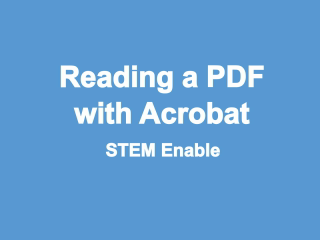
\includegraphics[width=0.6\linewidth,height=\textheight,keepaspectratio]{./Figs/Acrobat-thumbnail.png}

}

\caption{\href{https://www.youtube.com/watch?v=mgpo23i76O0}{Video
demonstration}\label{video}}

\end{figure}%

\subsection{Could we solve it by\ldots?}\label{could-we-solve-it-by}

Can we not solve this by ensuring that the PDF is accessible?
Unfortunately, the answer is currently, not yet\footnote{Work is ongoing
  to add encoding within a new PDF standard (PDF/UA-2 and WTPDF
  (Well-Tagged PDF) standards),
  \href{https://latex3.github.io/tagging-project/}{create a version of
  LaTeX which can do this} (itself, a multi-year project
  \href{https://latex3.github.io/tagging-project/documentation/}{currently
  in stage 4 of enabling package authors to apply changes}),
  \textbf{and} software which works with the extra encoding. The
  assistive technology vendors would then also need to support all of
  this. In the meantime we need to either convert the LaTeX to other
  formats or switch to a different scientific document preparation
  system.}. In current software and typically in-use PDF standards, the
act of creating the PDF destroys the structure of mathematical, and
similar, expressions. Reflow on a small screen produces\ldots{}

\begin{figure}[H]

{\centering 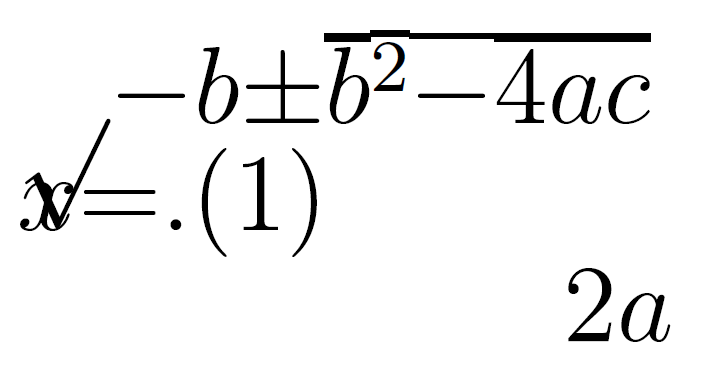
\includegraphics[width=0.4\linewidth,height=\textheight,keepaspectratio]{./Figs/reflowing.png}

}

\caption{Quadratic equation destroyed by reflow}

\end{figure}%

\section{What do solutions look
like?}\label{what-do-solutions-look-like}

\subsection{Structure + software}\label{structure-software}

Being able to adapt how text is presented, whether for small screens or
via assistive software requires:

\begin{itemize}
\tightlist
\item
  Authors to produce accessible materials which maintains the encoding
  of the structured text
\item
  Readers to have software and assistive technology which can manipulate
  the specific format
\end{itemize}

Until all this work is finished for PDF, only four formats of
mathematical text are technically accessible:

\begin{itemize}
\tightlist
\item
  HTML using MathJax to render the mathematics
\item
  Word/PowerPoint using the inbuilt equation editor
\item
  Word/PowerPoint using MathType
\item
  EPub3 using MathML
\end{itemize}

You \textbf{must} supply at least one to meet the public bodies
requirement.

\begin{itemize}
\tightlist
\item
  Supply your full course content `spine' in this format.
\end{itemize}

\subsection{So, job done?}\label{so-job-done}

Afraid not\ldots{}

Not all reader assistive technology can access maths in all formats!

\begin{itemize}
\tightlist
\item
  Equal access acts mean we must meet individual needs - so may need to
  produce other formats.
\item
  Some formats cannot not be transformed easily to others
\end{itemize}

For authors using Word/PowerPoint, standard accessiblity guidance is not
enough.

For authors using the LaTeX scientific document preparation system none
of the above formats are native outputs. \textbf{And} if a student can't
make their own clear print \textbf{and print it} you also may need to
supply variants on inaccessible PDF!

\begin{itemize}
\tightlist
\item
  Not all accessibility is about technical access
\item
  Clear print\footnote{Adhering as closely as possible to RNIB clear
    print guidelines} PDF is selected most often by disabled students in
  the Department of Mathematical Sciences at the University of
  Bath\footnote{Last year we had to assist an author to create a
    printable PDF for a disabled student after the author had made a
    whole (and completely technically accessible) course using ProTeXt -
    but couldn't get PDF working and the HTML produced poor print
    output\ldots{}}.
\end{itemize}

\section{How do you get started?}\label{how-do-you-get-started}

\subsection{Word/PowerPoint 365}\label{wordpowerpoint-365}

\begin{itemize}
\tightlist
\item
  Use the inbuilt Accessibility Checker and information on
  e.g.~\href{https://support.office.com/en-gb/article/make-your-word-documents-accessible-to-people-with-disabilities-d9bf3683-87ac-47ea-b91a-78dcacb3c66d}{Making
  your Word documents accessible}
\item
  Write \textbf{\emph{all}} mathematical text written using the MS 365
  equation editor. E.g. if you are writing about the variable (\(x\)) or
  (\(\theta\)) it should be written as an equation. If you are writing
  (\(x^2\)) it should be written as an equation.

  \begin{itemize}
  \tightlist
  \item
    Never use insert symbol.
  \item
    Never write superscripts, subscripts, fractions etc. using font or
    style changes and standard keyboard input alone
  \item
    Never use an image of an equation.
  \end{itemize}
\item
  Use Review -\textgreater{} Read Aloud (Alt + Ctrl + Space) to check
  the maths
\item
  \href{./example.docx}{Quick example}
\end{itemize}

\subsection{Word/PowerPoint transforms and
tools}\label{wordpowerpoint-transforms-and-tools}

\begin{itemize}
\tightlist
\item
  \href{https://bathmash.github.io/gettingstarted/Word/index.html}{Effective
  (keyboard-only) input of maths in Word}.
\item
  \href{https://www.cwu.edu/student-life/student-support/central-access/resources/reader.php}{Central
  Access Reader}

  \begin{itemize}
  \tightlist
  \item
    Transforms to specially set up HTML for screenreaders
  \item
    Can output MP3
  \item
    Can be used as text to speech software (but is not screenreader
    compatible)
  \end{itemize}
\item
  \href{https://www.wiris.com/en/mathtype/office-tools/}{Transform to
  MathType}

  \begin{itemize}
  \tightlist
  \item
    Student can convert to MathType - supply standard format
  \item
    Conversion back to Word is not possible in bulk
  \end{itemize}
\end{itemize}

At the time of writing transforming from (any) PowerPoint is tricky.
Best not to use this as a source format. If making slides, I would use
Quarto (used to make this!).

\subsection{HTML (WCAG 2.2 AA) +
MathJax!}\label{html-wcag-2.2-aa-mathjax}

\begin{itemize}
\item
  Check it meets the legal requirement of WCAG 2.2 Level AA with
  e.g.~\href{https://accessibilityinsights.io/docs/en/web/overview}{Accessibility
  Insights for Web plugin for Chrome}
\item
  Check it is MathJax\ldots{} Right click!
  \[x = \frac{-b\pm\sqrt{b^2 - 4ac}}{2a}\]

  \begin{itemize}
  \tightlist
  \item
    Provides/enables: navigation, chunking, zoom, copy/paste, colour,
    size and layout changes\ldots{}
  \item
    Encoded structure enables assistive technology including
    text-to-speech, screenreaders, electronic Braille
  \item
    Fallback for ARIA-aware AT without native support
  \item
    AT providers without native support and not ARIA aware are a problem
    but not your problem.
  \end{itemize}
\end{itemize}

We recommend using MathJax 2.7.9 or
\href{https://docs.mathjax.org/en/v4.0/output/linebreaks.html}{MathJax
4.* as MathJax 3.* does not enable reflow on zoom} (a requirement for
WCAG 2.2 AA).

\subsection{Scientific document preparation
systems}\label{scientific-document-preparation-systems}

\begin{itemize}
\tightlist
\item
  Attempt to transform the LaTeX\footnote{It is \textbf{not possible} to
    convert LaTeX to html in the general case. It is easy to `fall out'
    of the convertible subset without realising or knowing why, the
    addition of a package, change of preamble order, use of a seemingly
    innocent command\ldots{}} to HTML with MathJax using
  \href{https://chirun.org.uk/}{Chirun},
  \href{https://vlmantova.github.io/bookml/}{BookML} or
  \href{https://ctan.org/pkg/lwarp?lang=en}{lwarp}

  \begin{itemize}
  \tightlist
  \item
    What happens depends on what you are doing in LaTeX
  \item
    Keep your preamble \textbf{clean}, start with a minimal document,
    add in sections recompiling to all required output formats after
    each addition
  \item
    Some documents cannot be converted
  \item
    \textbf{I don't know of a Beamer solution} at time of writing
  \end{itemize}
\item
  Work in a Markdown format, using LaTeX for equations, with HTML has
  the primary output (can also output LaTeX/PDF); can create slides and
  single-source slides and documents (like Beamer)

  \begin{itemize}
  \tightlist
  \item
    \href{https://quarto.org/}{Quarto} is recommended in most cases

    \begin{itemize}
    \tightlist
    \item
      \href{https://bookdown.org/}{Bookdown} continues to be fine but
      start new projects in Quarto
    \end{itemize}
  \item
    \href{https://rmarkdown.rstudio.com/}{RMarkdown} can be a helpful
    starting point for those completely new
  \item
    \href{https://bathmash.github.io/clavertondown/}{Clavertondown},
    built using RMarkdown and Bookdown; only if other methods can't meet
    needs
  \end{itemize}
\end{itemize}

\subsection{Non-text elements}\label{non-text-elements}

\begin{itemize}
\tightlist
\item
  Graphical elements

  \begin{itemize}
  \tightlist
  \item
    \href{https://www.desmos.com/accessibility}{Desmos was designed to
    work and tested with screenreaders and written to conform to WCAG
    2.1}
  \item
    \href{https://www.geogebra.org/m/r2EF8uRx}{Geogebra aims to meet
    WCAG 2.1 AA}
  \item
    \href{https://bathmash.github.io/CETL-MSOR-2022-Beyond-alt-text/index.html}{Project
    \textbf{Beyond alt text} between Bath and Coventry produced
    guidelines}
  \item
    \href{https://github.com/ajrgodfrey/BrailleR}{BrailleR} is a project
    by and for \href{https://r-resources.massey.ac.nz/BrailleR/}{blind
    statisticians who use R}
  \item
    \href{http://diagramcenter.org/}{DIAGRAM Center} has some great
    resources for those new to diagram description:

    \begin{itemize}
    \tightlist
    \item
      Poet Image Description Training Tool
    \item
      Image description guidelines
    \item
      Sample book
    \item
      \href{http://diagramcenter.org/diagramwebinars.html\#compleximages}{Webinar
      on complex images}
    \end{itemize}
  \end{itemize}
\item
  Maths e-assessment

  \begin{itemize}
  \tightlist
  \item
    \href{https://docs.numbas.org.uk/en/latest/accessibility/editor.html}{Numbas
    aims to meet WCAG 2.1 AA}
  \item
    \href{https://stack-assessment.org/Legal/Accessibility/}{Stack aims
    to meet WCAG 2.1 AA}
  \end{itemize}
\end{itemize}

\section{Next steps}\label{next-steps}

The ideal can feel a long way off\ldots{}

\begin{itemize}
\tightlist
\item
  Pick a place to start which feels achievable and start!
\item
  The journey is less lonely if we share experiences and learn from each
  other

  \begin{itemize}
  \tightlist
  \item
    Consider setting up an institution community of practice, after 6
    years our Markdown/Bookdown/ClavertonDown/Quarto CoP answers many
    questions between themselves without help from me, my team or the
    specialist STEM learning technologists (who we are very lucky to
    have)
  \item
    In the UK there is the
    \href{https://sites.google.com/view/accessible-maths/home}{JISC
    Accessibility Community Maths Working Group}.

    \begin{itemize}
    \tightlist
    \item
      Is there anything similar in Ireland?
    \item
      It may be worth exploring whether links can be made with them from
      Ireland
    \end{itemize}
  \end{itemize}
\end{itemize}

Want to see how I built this single-source, multiple-outputs document?
\href{https://github.com/STEM-Enable/Quick-introduction-to-accessible-maths-2026/}{Github
repository source - see qmd file}

Here is some text which is only included in the notes formats!

\begin{itemize}
\tightlist
\item
  To prove it is possible to create slides and notes from one source
\item
  You will find this part only in the html document and the Word format,
  not in any of the slide formats
\end{itemize}




\end{document}
